\documentclass[12pt,subeqn]{article}

%\usepackage[dvips]{graphicx}
\usepackage[latin1]{inputenc}
\usepackage{graphicx}
\usepackage{psfrag}
\usepackage{amssymb}
\usepackage{amsmath}
\usepackage{amsfonts}
\usepackage{epstopdf}
\usepackage{array}
\usepackage{latexsym}
\usepackage{subfig}
\usepackage{float}
\usepackage{enumitem}
\usepackage[pdftex,bookmarks,colorlinks]{hyperref}
\usepackage[notcite,notref]{showkeys}
\numberwithin{equation}{section} 
\makeatletter
\@ifundefined{showcaptionsetup}{}{%
 \PassOptionsToPackage{caption=false}{subfig}}
\usepackage{subfig}
\makeatother

\usepackage{calc}
\usepackage{amsthm}
\usepackage[usenames,dvipsnames]{xcolor}
\usepackage{tikz}
\usepackage[all]{xy}
\usetikzlibrary{shapes,arrows,decorations.pathreplacing, calc}
\makeatletter
\newcommand{\gettikzxy}[3]{%
  \tikz@scan@one@point\pgfutil@firstofone#1\relax
  \edef#2{\the\pgf@x}%
  \edef#3{\the\pgf@y}%
}
\makeatother
%\DeclareGraphicsRule{.tif}{png}{.png}{`convert #1 `dirname #1`/`basename #1 .tif`.png}

%\textwidth = 6.5 in
%\textheight = 9 in
%\oddsidemargin = 0.0 in
%\evensidemargin = 0.0 in
%\topmargin = 0.0 in
%\headheight = 0.0 in
%\headsep = 0.0 in
%\parskip = 0.2in
%\parindent = 0.0in

\newtheorem{theorem}{Theorem}
\newtheorem{lemma}[theorem]{Lemma}
\newtheorem{corollary}{Corollary}
\newtheorem{prop}{Proposition}
\newtheorem{definition}{Definition}[section]
\newtheorem{remark}{Remark}
\newtheorem{example}{Example}
\newtheorem{notation}{Notation}

%\newenvironment{proof}{\smallskip\noindent\emph{Proof.}\hspace{1pt}}%
%{\hspace{-5pt}{\nobreak\quad\nobreak\hfill\nobreak$\square$\vspace{8pt}%
%\par}\smallskip\goodbreak}

\newcommand{\R}{\mathbb R}
\newcommand{\Riem}{\mathcal{RS}}
\newcommand{\Rieml}{\Riem_{\bar{l}}}
\newcommand{\tv}{\hbox{\textrm{TV}}}
\newcommand{\BV}{\hbox{\textrm{BV}}}
\newcommand{\N}{{\mathbb N}}
\newcommand{\CC}{{\mathcal C}}
\newcommand{\Z}{\mathbb{Z}}
\newcommand{\dt}{{\Delta t}}
\newcommand{\dx}{{\Delta x}}
\newcommand{\xjmudemi}{x_{j-1/2}}
\newcommand{\xjpudemi}{x_{j+1/2}}
\newcommand{\OO}{\mathcal{O}}

\newcommand{\del}{\partial}

\newcommand{\be}{\begin{equation}}
\newcommand{\ee}{\end{equation}}

\newcommand{\modulo}[1]{{\left|#1\right|}}
\newcommand{\norma}[1]{{\left\|#1\right\|}}

\renewcommand{\L}[1]{\mathbf{L^#1}}
\newcommand{\Lloc}[1]{\mathbf{L^{#1}_{loc}}}
\newcommand{\C}[1]{\mathbf{C^{#1}}}
\newcommand{\Cc}[1]{\mathbf{C_c^{#1}}}



%\DeclareMathOperator{\argmin}{argmin}
\DeclareMathOperator{\sgn}{sgn}
%\DeclareMathOperator{\proj}{Proj}


\begin{document}

\title{Traffic flow modeling: a highway ramp model.}
\author{...}

\maketitle

\section{Introduction}
We consider a junction with one incoming mainline modeled by the real interval $]-\infty,0]$ and an outgoing mainline modeled by the interval $[0,+\infty[$, one onramp and one offramp, see Figure \ref{fig:junction}.
\begin{figure}[H]
\centering
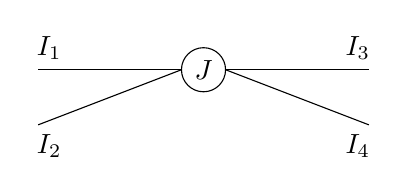
\begin{tikzpicture}[scale=1.4]
\draw (-1.5,0)--(-0.2,0);
\draw (0,0) circle (0.2);
\draw (0.2,0)--(1.5,0);
\draw (-0.2,0)--(-1.5,-0.5);
\draw (0.2,0)--(1.5,-0.5);
\node at (0,0) {$J$};
\node [above] at (-1.4,0) {$I_1$};
\node [above] at (1.4,0) {$I_3$};
\node [below] at (-1.4,-0.5) {$I_2$};
\node [below] at (1.4,-0.5) {$I_4$};
\end{tikzpicture}
\caption{Junction taken into consideration.}
\label{fig:junction}
\end{figure}
From a macroscopic point of view this means that on each mainline road $I_1=]-\infty ,0[$ and $I_2=]0,+\infty [$ we consider the equation
\be
	\del_t \rho + \del_x f(\rho) =0, \quad  (t,x)\in\R^+\times\R, 
	\label{eq:LWR}
\ee
where $\rho=\rho(t,x) \in [0, \rho_{max}]$ is the density of the cars on each mainline, $v \geq 0$ is the mean traffic speed in free flow, $w\leq 0$ is the mean traffic speed in congested flow, i.e. the slope of the line representing the congested flow in the fundamental diagram and \\ $f(\rho) =
	\left\{
	\begin{array}{ll}
		v\rho &\hbox{if}~\rho\leq\rho^{cr} , \\
		w(\rho-\rho_{max}) &\hbox{otherwise},
	\end{array}
	\right.$ \quad is the flux.\\ \\
We assume the following:
\begin{itemize}
	\item[] (A1) $\rho_{max}=1$;
	\item[] (A2) $f(0)=f(1)=0$;
	\item[] (A3) the flux is a strictly concave function.
\end{itemize}
Moreover we consider a triangular fundamental diagram, see Figure \ref{fig:FDiag}.
\begin{figure}[H]
\centering
\begin{tikzpicture}[scale=1.4]
\draw [<->] (0,3) -- (0,0) -- (4,0);
\draw (0,0)--(1.5,2);
\draw (1.5,2)--(3.5,0);
\draw [dashed] (1.5,2)--(0,2); 
\draw [dashed] (1.5,2)--(1.5,0);
\draw [dashed, line width=0.1mm] (0.5,0.6)--(1,0.6);
\draw [dashed, line width=0.1mm] (1,1.3)--(1,0.6);
\draw [dashed, line width=0.1mm] (2.9,0.6)--(2.2,0.6);
\draw [dashed, line width=0.1mm] (2.2,1.3)--(2.2,0.6);
\node [below] at (3.9,0) {$\rho$};
\node [below] at (1.5,0) {$\rho^{cr}$};
\node [left] at (0,2) {$f^{max}$};
\node [left] at (0,3) {$f(\rho)$};
\node [right] at (1,1) {$v$}; 
\node [left] at (2.2,1) {$w$};
\end{tikzpicture}
\caption{Triangular fundamental diagram}
\label{fig:FDiag}
\end{figure}

On the onramp $R_1$ we consider the presence of a buffer modeled with the following ODE:
\be
	\dfrac{dl(t)}{dt}=F_{in}(t)-\gamma_{r1}(t), \quad t\in\R^+ ,
	\label{eq:ODEonramp}
\ee
where $l(t) \in [0, +\infty[$ is the load on the buffer, $F_{in}(t)$ is the flux that enters the onramp and $\gamma_{r1}(t)$ is the flux that exits from the onramp. \\
This particular choice was made to avoid backward waves on the onramp boundary which happens in the case of horizontal queues.

The Cauchy problem to solve is then:
\be
	\label{eq:CP}
		\left\{
		\begin{array}{ll}
		\del_t \rho_i + \del_x f(\rho_i) =0, & (t,x)\in\R^+\times I_i, \\
		\dfrac{dl(t)}{dt}=F_{in}(t)-\gamma_{r1} (t), & t\in\R^+ ,\\
		\rho_i(0,x)=\rho_{i,0}(x), & \text{on } I_i \\
		l(0)=l_0,
		\end{array}
		\right.
\ee
where $l_0 \in [0,+\infty[$ is the initial load of the buffer. 
We consider the offramp as an infinite sink that accept all the flux that comes to it from the mainline $I_1$.\\
This will be coupled with the following problem at the junction which will give the distribution of the traffic among the roads:\\
 \begin{eqnarray}
 	\label{eq:JunctionProblem}
		&d(t)&=\left\{
			 \begin{array}{ll}
			 \gamma^{max}_{r1} &\hbox{if}~l(t)>0 , \\ 
			 \min{(F_{in}(t),\gamma_{r1}^{max})} &\hbox{if}~l(t)=0,
			 \end{array}
			 \right.\\ \nonumber
		&\delta(t)&=\min{(f^{max},v\rho_1)},	 \\ \nonumber
		&\sigma(t)&=\min{(f^{max},w(\rho_2 - \rho_{max}))},\\ \nonumber
		&\gamma_{r2}(t)&=\beta f_{1}(\rho(t,0-)),	\\ \nonumber	
		&f_{2}(t,0+)&=\min{((1-\beta)\delta(t)+d(t), \sigma(t))},
\end{eqnarray}
where $\gamma_{r1}^{max}$ is the maximal flow on the onramp, $\delta(t)$ is the demand function on the mainline, $d(t)$ is the demand of the onramp, $f^{max}$ the maximal flux on $I_1$ and $I_2$, $\sigma(t)$ is the supply function on $I_2$ and $\beta \in [0,1]$ is the split ratio of the offramp.\\ 
Denote with $\rho_i:[0, +\infty[\times I_i \rightarrow [0,1]$ the density of the cars in the road $I_i$ of the junction. We want $\rho_i$ to be a weak solution on $I_i$, i.e. for all $\varphi \in \CC^1_c(\R^+ \times I_i)$
\be
	\int_{\R^+}\int_{\R}\Big( \rho_i \del_t\varphi +f(\rho_i)\del_x\varphi \Big)dxdt=0
	\label{eq:weakSolRhoi}
\ee

\begin{definition}
	\label{def:weakSolRho}
	Let $J$ be a junction with one incoming road $I_1$ and one outgoing road $I_2$. A weak solution at $J$ is a couple of functions $\rho_i :[0,+\infty[ \times I_i \rightarrow \R$, $i=1,2$, such that 
	\begin{eqnarray}	
		\Big(\int_{\R^+}\int_{I_1}\Big( \rho_1 \del_t\varphi_1 +f(\rho_1)\del_x\varphi_1 \Big)dxdt\Big)=0, \nonumber \\
		\Big(\int_{\R^+}\int_{I_2}\Big( \rho_2 \del_t\varphi_2 +f(\rho_2)\del_x\varphi_2 \Big)dxdt\Big)=0,		
		\label{eq:weakSolRho}
	\end{eqnarray}
	for every $\varphi_i \in \CC^1_c(\R^+\times I_i)$. 
\end{definition}
\begin{remark}
	The fluxes $f_1(\rho(t,0-))$, $f_2(\rho(t,0+))$,$\gamma_{r1}(t)$ and $\gamma_{r2}(t)$ must satisfy the Rankine-Hugoniot condition:
	\begin{equation}
		f_1(\rho(t,0-))+\gamma_{r1}(t)=f_2(\rho(t,0+))+\gamma_{r2}(t).
		\label{eq:conservationAtJ}
	\end{equation}
\end{remark}
\begin{definition}
	\label{def:weak_sol}
	A collection of functions $(\rho_1,\rho_2,l)\in \prod_{i=1}^2 \CC^0\left( \R^+; \L1\cap\BV (\R)\right) \times \mathbf{W^{1,\infty}}(\R^+;\R^+)$ is a solution at $J$ to (\ref{eq:CP}) if
	\begin{enumerate}[label=(\roman{*}),ref=(\roman{*})]
		\item \label{item:i} $\rho_1$,$\rho_2$ are weak solutions on $I_1$, $I_2$, i.e., see Definition \ref{def:weakSolRho};
		\item \label{item:ii} $f_1(\rho(t,0-))=\dfrac{P}{1-P}\gamma_{r1}$ with $P \in ]0,1[$ the priority factor;
		\item \label{item:iii} $f_1(\rho(t,0-))+\gamma_{r1}(t)=f_2(\rho(t,0+))+\gamma_{r2}(t)$; 
		\item \label{item:iv} $f_2(\rho(t,0+))$ is maximum subject to \ref{item:ii},\ref{item:iii} and \eqref{eq:JunctionProblem};
		\item \label{item:v} $l$ is a solution of the ODE \eqref{eq:ODEonramp} for a.e. $t\in\R^+$.		
	\end{enumerate}
\end{definition}
\begin{remark}
	The priority factor $P$ is introduced to ensure the uniquess of the solution which was not guaranteed only with the maximization of the flow $f_2(\rho(t,0+))$.
\end{remark}
\section{The Riemann problem at the junction}
In this section we construct step by step the Riemann Solver ($\mathcal{RS}$) at the junction.
Fix $\rho_{1,0},\rho_{2,0} \in [0,1]$, $l_0 \in [0,+\infty[$ and a priority factor $P \in ]0,1[$. The Riemann problem at $J$ is the Cauchy problem \eqref{eq:CP} where the initial conditions are given by $\rho_{0,i}(x)\equiv \rho_{0,i} $ in $I_i$ for every $i=1,2$. We define the Riemann Solver by means of a Riemann Solver $\Rieml$, which depends on the instantaneous load of the buffer $\bar{l}$. For each $\bar{l}$ the Rieman Solver $\Rieml$ is constructed in the following way.
\begin{enumerate}
	\item Define $\Gamma_1=f_1(\rho_1(t,0-))$, $\Gamma_2=f_2(\rho_2(t,0+))$, $\Gamma_3=\gamma_{r1}(t)$;
	\item Consider the space ($\Gamma_1$,$\Gamma_3$) and the sets $\OO_1=[0,\delta(t)]$, $\OO_3=[0,d(t)]$;
%	\item Define the set $$\bar{\Omega}_3=\left\{
%			 \begin{array}{ll}
%			 [0,\Gamma_3^{max}] &\hbox{if}~\bar{l}>0 , \\ 
%			 \left[0,\min{(\Gamma_3^{max},F_{in})}\right] &\hbox{if}~\bar{l}=0;
%			 \end{array}
%			 \right. $$;
	\item Trace the lines $(1-\beta)\Gamma_1+\Gamma_3=\Gamma_2$ and $\Gamma_1=\frac{P}{1-P}\Gamma_3$;
	\item Define $Q$ to be the point of intersection of the two lines; 
	\item Consider the region $$\Omega=\Big\{  (\Gamma_1,\Gamma_3) \in \OO_1 \times \OO_3 : (1-\beta)\Gamma_1+\Gamma_3 \in [0,\Gamma_2]  \Big\} .$$ 
\end{enumerate}
Two situations can occur at this point:
\begin{itemize}
	\item $Q$ belongs to $\Omega$,
	\item $Q$ is outside $\Omega$.
\end{itemize}
In the first case we set ($\hat{\Gamma}_1$,$\hat{\Gamma}_3$)=$Q$, while in the second case we set ($\hat{\Gamma}_1$,$\hat{\Gamma}_3$)=$S$ where $S$ is the point of the segment $\Omega \cap {(\Gamma_1,\Gamma_3): (1-\beta)\Gamma_1+\Gamma_3=\Gamma_2}$ closest to the line $\Gamma_1=\frac{P}{1-P}\Gamma_3$. We show in Figure \ref{fig:junctionRS} the different cases that can occur.
\begin{figure}[h]
\centering
\subfloat[Intersection inside $\Omega$]{
\resizebox{.33\columnwidth}{!}{
	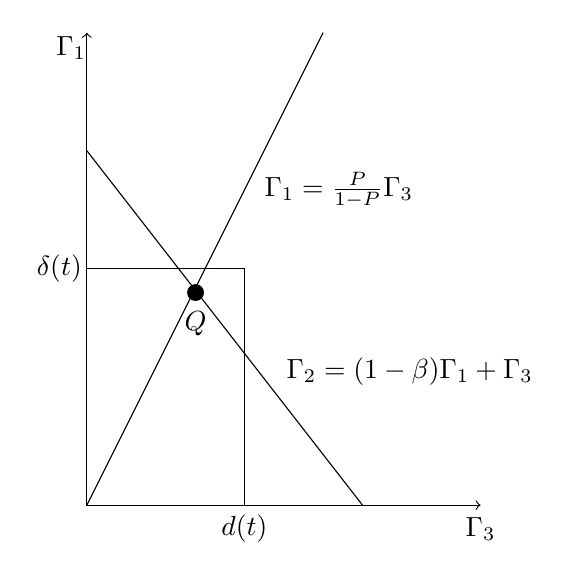
\begin{tikzpicture}
	\draw[<->] (0,6) -- (0,0) --(5,0);
	\draw (0,0) rectangle (2,3);
	\draw (3.5,0) -- (0,4.5);
	\draw (0,0) -- (1,2)--(3,6);
	\draw[fill=black](1.38,2.7) circle (0.1);
	\node (below) at (5,-0.3) {$\Gamma_3$};
	\node (below) at (2,-0.3) {$d(t)$};
	\node (left) at (-0.2,5.8) {$\Gamma_1$};
	\node (left) at (-0.35,3) {$\delta(t)$};
	\node (right) at (4.1,1.7) {$\Gamma_2=(1-\beta)\Gamma_1 +\Gamma_3$};
	\node (right) at (3.2,4) {$\Gamma_1=\frac{P}{1-P}\Gamma_3$};
	\node (below) at (1.38,2.3) {$Q$};
\end{tikzpicture}

}
\label{fig:solution}
}
\subfloat[Intersection outside $\Omega$]{
\resizebox{.33\columnwidth}{!}{
	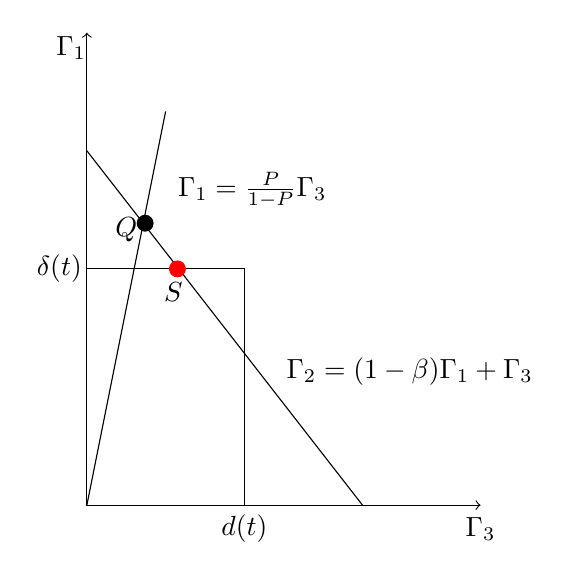
\begin{tikzpicture}
	\draw[<->] (0,6) -- (0,0) --(5,0);
	\draw (0,0) rectangle (2,3);
	\draw (3.5,0) -- (0,4.5);
	\draw (0,0) -- (0.5,2.5) -- (1,5);
	\draw[fill=black](0.74,3.58) circle (0.1);
	\draw[color=red, fill=red](1.15,3) circle (0.1);
	\node (below) at (5,-0.3) {$\Gamma_3$};
	\node (below) at (2,-0.3) {$d(t)$};
	\node (left) at (-0.2,5.8) {$\Gamma_1$};
	\node (left) at (-0.35,3) {$\delta(t)$};
	\node (right) at (4.1,1.7) {$\Gamma_2=(1-\beta)\Gamma_1 +\Gamma_3$};
	\node (right) at (2.1,4) {$\Gamma_1=\frac{P}{1-P}\Gamma_3$};
	\node (left) at (0.5,3.5) {$Q$};
	\node (below) at (1.1,2.7) {$S$};
\end{tikzpicture}
}
\label{fig:solution2}
}
\subfloat[Intersection outside $\Omega$]{
\resizebox{.33\columnwidth}{!}{
	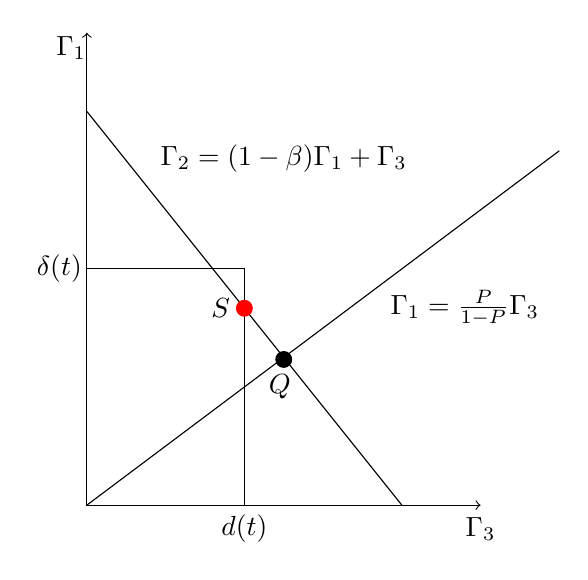
\begin{tikzpicture}
	\draw[<->] (0,6) -- (0,0) --(5,0);
	\draw (0,0) rectangle (2,3);
	\draw (4,0) -- (0,5);
	\draw (0,0) -- (4,3) -- (6,4.5);
	\draw[fill=black](2.5,1.85) circle (0.1);
	\draw[color=red, fill=red](2,2.5) circle (0.1);
	\node (below) at (5,-0.3) {$\Gamma_3$};
	\node (below) at (2,-0.3) {$d(t)$};
	\node (left) at (-0.2,5.8) {$\Gamma_1$};
	\node (left) at (-0.35,3) {$\delta(t)$};
	\node (right) at (2.5,4.4) {$\Gamma_2=(1-\beta)\Gamma_1 +\Gamma_3$};
	\node (right) at (4.8,2.5) {$\Gamma_1=\frac{P}{1-P}\Gamma_3$};
	\node (below) at (2.45,1.5) {$Q$};
	\node (left) at (1.7,2.5) {$S$};
\end{tikzpicture}
}
\label{fig:solution3}
}
\caption{Solutions Riemann Solver at the junction}
\label{fig:junctionRS}
\end{figure}\\
Note that in the second case it is not possible to respect in an exact way the priority given by the parameter $P$ if we want to maximize also the flux. So we solve in this case the minimization problem
\begin{equation}
	\begin{aligned}
		{\text{minimize}}
		& &  \Big\|  \left( \begin{array}{c}
							\gamma_{r1}(t) \\
							f_{1}(\rho_1(t,0-)) 
							\end{array} \right)- \left( \begin{array}{c}
															\gamma_{r1}(t) \\
															f_{1}(\rho_1(t,0-)) 
															\end{array} \right) \cdot \alpha^P \alpha^P \Big\|^2_2 \\
		\vspace{1pt}															
		\text{subject to}
		& & f_{2}(\rho_2(t,0+)) = (1-\beta)f_{1}(\rho_1(t,0-)) + \gamma_{r1}(t),\\
		& & \gamma_{r1}(t) \leq d(t),\\
		& & f_{1}(\rho_1(t,0+)) \leq \delta(t),
	\end{aligned}
	\label{eq:minimizationP}
\end{equation}
where $\alpha^P$ is the normalized vector $\alpha^P=\dfrac{1}{\sqrt{P^2+(1-P)^2}}\left( \begin{array}{c}
							P \\
							1-P 
							\end{array} \right)$ with $P$ the priority factor.\\
Once we have determined $\hat{\Gamma}_1$ and $\hat{\Gamma}_2$ we can determine in an unique way $\hat{\rho}_1$, $\hat{\rho}_2$ as follows. \\
We recall that $\rho=\rho^{cr}\in]0,1[$ is the unique point of maximum of the flux and we define the function $\tau$ as follows.
\begin{definition}
	Let $\tau:[0,1]\rightarrow[0,1]$ be the map such that:
	\begin{itemize}
		\item $f(\tau(\rho))=f(\rho)$ for every $\rho\in [0,1]$;
		\item $\tau(\rho)\neq\rho$ for every $\rho\in[0,1]\setminus\{\rho^{cr}\}$
	\end{itemize}
\end{definition}
For the function $\tau$ in this context is valid \cite[Proposition 4.3.2.]{garavello2006traffic}.\\
Given $$\rho_1(0,\cdot)\equiv \rho_{1,0}\text{ , }\rho_2(0,\cdot)\equiv \rho_{2,0} $$ there exists a unique couple $(\hat{\rho}_1 ,\hat{\rho}_2)\in[0,1]^2$ such that
	\begin{equation}
		\hat{\rho}_1\in\left\{
		\begin{array}{ll}
		\{\rho_{1,0}\}\cup]\tau(\rho_{1,0}),1] &\hbox{if}~0 \leq \rho_{1,0}\leq\rho^{cr} ,\\
		\left[\rho^{cr},1\right] &\hbox{if}~\rho^{cr} \leq \rho_{1,0}\leq 1;
		\end{array}
		\right.
		\label{eq:rho_1}
	\end{equation}
	and
	\begin{equation}
		\hat{\rho}_2\in\left\{
		\begin{array}{ll}
		\left[0,\rho^{cr}\right] &\hbox{if}~0 \leq \rho_{2,0}\leq\rho^{cr} ,\\		
		\{\rho_{2,0}\}\cup[0,\tau(\rho_{2,0})[ &\hbox{if}~\rho^{cr} \leq \rho_{1,0}\leq 1;
		\end{array}
		\right.
		\label{eq:rho_2}
	\end{equation}
and for the incoming road the solution is given by the wave $(\rho_{1,0},\hat{\rho}_1)$, while for the outgoing road the solution is given by the wave $(\hat{\rho}_2,\rho_{2,0})$.
%Therefore the following theorem holds.
%\begin{theorem}
%	\label{th:existenceSol}
%	Consider a junction $J$ and fix a priority parameter $P \in  ]0,1[$. For every $\rho_{1,0}$,$\rho_{2,0} \in [0,1]$, there exists a unique admissible solution $\rho=(\rho_1,\rho_2)$ to \eqref{eq:LWR} at the junction J in the sense of Definition \ref{def:weak_sol_Junct} such that $$\rho_1(0,\cdot)\equiv \rho_{1,0}\text{ , }\rho_2(0,\cdot)\equiv \rho_{2,0} $$.\\
%	Moreover, there exists a unique couple $(\hat{\rho}_1 ,\hat{\rho}_2)\in[0,1]^2$ such that
%	\begin{equation}
%		\hat{\rho}_1\in\left\{
%		\begin{array}{ll}
%		\{\rho_{1,0}\}\cup]\tau(\rho_{1,0}),1] &\hbox{if}~0 \leq \rho_{1,0}\leq\rho^{cr} ,\\
%		\left[\rho^{cr},1\right] &\hbox{if}~\rho^{cr} \leq \rho_{1,0}\leq 1;
%		\end{array}
%		\right.
%		\label{eq:rho_1}
%	\end{equation}
%	and
%	\begin{equation}
%		\hat{\rho}_2\in\left\{
%		\begin{array}{ll}
%		\left[0,\rho^{cr}\right] &\hbox{if}~0 \leq \rho_{2,0}\leq\rho^{cr} ,\\		
%		\{\rho_{2,0}\}\cup[0,\tau(\rho_{2,0})[ &\hbox{if}~\rho^{cr} \leq \rho_{1,0}\leq 1;
%		\end{array}
%		\right.
%		\label{eq:rho_2}
%	\end{equation}
%and for the incoming road the solution is given by the wave $(\rho_{1,0},\hat{\rho}_1)$, while for the outgoing road the solution is given by the wave $(\hat{\rho}_2,\rho_{2,0})$.
%\end{theorem}
In this setting, given the initial data $\rho_{1,0}$, $\rho_{2,0}$ we can define $\Rieml:[0,1]^2\rightarrow[0,1]^2$ by 
\begin{equation}
	\label{eq:Rieml}
	\Rieml(\rho_{1,0},\rho_{2,0})=(\hat{\rho}_1 ,\hat{\rho}_2 , \hat{\Gamma}_3 ).
\end{equation}
Now given the initial load of the buffer $l_0=\bar{l}$, the function $l(t)$ at time $t>0$ is given by
\begin{equation}
	\label{eq:solODE}
	l(t)=\left\{
			 \begin{array}{ll}
			 l_0 + (F_{in} - \hat{\Gamma}_3)t &\hbox{if}~ 0 < t < -\frac{l_0}{F_{in} - \hat{\Gamma}_3},\\ 
			 0 &\hbox{if}~t > -\frac{l_0}{F_{in} - \hat{\Gamma}_3},
			 \end{array}
			 \right.
\end{equation}
%The solution for the Riemann problem is given by the unique solution at $J$ $(\rho_1(t,x),\rho_2(t,x),l(t))$ in the sense of Definition \ref{def:weak_sol}, such that for a.e. $t>0$ it holds
%$$(\rho_1(t,0),\rho_2(t,0))=\Riem_{l(t)}(\rho_1(t,0),\rho_2(t,0))$$. 
\begin{remark}
The presence of the buffer can create waves at time $\bar{t} > 0$. In particular, we have a new wave if $F_{in} < \hat{\Gamma}_3$ and the buffer empties, see Figure  \ref{fig:RiemProb}. \\
No waves are created instead in the other case due to the infinity capacity of the buffer.
\end{remark}
\begin{figure}[H]
\centering
\begin{tikzpicture}[scale=0.8]
	\draw[<-] (0,6) -- (0,0);
	\draw[->] (-6,0) -- (6,0);	
	\draw (0,0) -- (2,2)--(6,6);
	\draw (0,0) -- (-2,2)--(-6,6);
	\draw (0,3) -- (2,6);
	\node (left) at (-0.2,3.1) {$\bar{t}$};	
	\node (left) at (-0.2,5.85) {$t$};
	\node (below) at (5.9,-0.3) {$x$};
	\node (below) at (0,-0.3) {$0$};
	\node (above) at (-3,1) {$\rho_{1,0}$};
	\node (above) at (3,1) {$\rho_{2,0}$};
	\node (above) at (-3,4) {$\hat{\rho}_1$};
	\node (above) at (3,4) {$\hat{\rho}_2$};
	\node (above) at (0.5,5) {$\bar{\rho}_2$};
\end{tikzpicture}

\caption{Solution of the Riemann Problem}
\label{fig:RiemProb}
\end{figure}
The following theorem holds.
\begin{theorem}
	\label{th:existenceSol}
	Consider a junction $J$ and fix a priority parameter $P \in  ]0,1[$. For every $\rho_{1,0}$,$\rho_{2,0} \in [0,1]$ and $l_0 \in [0, +\infty]$, there exists a unique admissible solution $(\rho_1(t,x),\rho_2(t,x),l(t))$ in the sense of Definition \ref{def:weak_sol} such that for a.e. $t>0$ it holds
$$(\rho_1(t,0-),\rho_2(t,0+))=\Riem_{l(t)}(\rho_1(t,0-),\rho_2(t,0+))$$. 
\end{theorem}
\begin{proof}
	Self-similarity
\end{proof}

%\section{The Riemann problem at the junction}
%In this section we construct step by step the Riemann Solver ($\mathcal{RS}$) at the junction.
%We assume a priority parameter that governs the access to the outgoing mainline $I_2$ and we fix with $Pf_{I_1}(t,0-)$ the cars coming from the first incoming road and with $(1-P)f_{O_1}(t,0-)$ the cars coming from the onramp, with $P \in ]0,1[$. We want to maximize the flux going through the junction. We suppose initial data in the mainline equal to $\rho_{1,0}$ and $\rho_{2,0}$. We consider the buffer initially empty, i.e. $l_0=0$. In the following, for simplicity we will consider $\gamma_1=f_{I_1}(t,0-)$, $\gamma_2=f_{I_2}(t,0+)$, $\gamma_3=f_{O_1}(t,0-)$ and $\hat{\gamma}_1$, $\hat{\gamma}_2$ and $\hat{\gamma}_3$ the corresponded solutions. In this context the Riemann problem will depends instantaneously on the load of the buffer $\bar{l}$
%\begin{enumerate}
%	%\item Define the sets $\Omega_{I_1}=[0,\delta(t)]$, $\Omega_{O_1}=[0,d(t)]$, $\Omega_{I_2}=[0,\sigma(t)]$, $\Omega_{O_2}=[0,+\infty]$, $\Omega=\{f_{I_1}(t,0-), f_{O_1}(t,0-)\in\Omega_{I_1} \times \Omega_{O_1} | (\frac{P}{1-P}\cdot f_{O_1}(t,0-),f_{I_2}(t,0+)) \in \Omega_{I_2} \times \Omega_{O_2}\}$.\\ The set $\Omega$ is closed, convex and not empty.
%	\item  Consider the space ($\gamma_1$,$\gamma_3$) and the sets $\Omega_1=[0,\delta(t)]$, $\Omega_3=[0,d(t)]$;
%	\item Define the set $$\bar{\Omega}_3=\left\{
%			 \begin{array}{ll}
%			 [0,f_{O_1}^{max}] &\hbox{if}~\bar{l}>0 , \\ 
%			 \left[0,\min{(f_{O_1}^{max},f_{O_1}(\rho(t,-\infty)))}\right] &\hbox{if}~\bar{l}=0;
%			 \end{array}
%			 \right. $$
%	\item Trace the lines $(1-\beta)\gamma_1+\gamma_3=\gamma_2$ and $\gamma_1=\frac{P}{1-P}\gamma_3$;
%	\item Define $Q$ to be the point of intersection of the two lines; 
%	\item Consider the region $$\Omega=\Big\{  (\gamma_1,\gamma_3):\gamma_1,\gamma_3 \in \Omega_1 \times \bar{\Omega}_3, (1-\beta)\gamma_1+\gamma_3 \in [0,\gamma_2]  \Big\} $$.
%\end{enumerate}
%Two situations can occur at this point:
%\begin{itemize}
%	\item $Q$ belongs to $\Omega$,
%	\item $Q$ is outside $\Omega$.
%\end{itemize}
%In the first case we set ($\hat{\gamma}_1$,$\hat{\gamma}_3$)=$Q$, while in the second case we set ($\hat{\gamma}_1$,$\hat{\gamma}_3$)=$S$ where $S$ is the point of the segment $\Omega \cap {(\gamma_1,\gamma_3): (1-\beta)\gamma_1+\gamma_3=\gamma_2}$ closest to the line $\gamma_1=\frac{P}{1-P}\gamma_3$ as enforced by the minimization problem \ref{eq:minimizationP}. With this we are able to find $\hat{\rho}_1$ and $\hat{\rho}_2$ from the values of $\hat{\gamma}_1$,$\hat{\gamma}_2$
%At this point we are able to define $\mathcal{RS}:[0,1]^{2}\rightarrow[0,1]^{2}$ by
%\be
%	\mathcal{RS}(\rho_{1,0},\rho_{2,0})=(\hat{\rho_{1}},\hat{\rho_2}).
%	\label{eq:RS}
%\ee
%Now given the initial load $l_0$ of the buffer and denoting with $$\Delta=\left\{
%			 \begin{array}{ll}
%			 f_{O_1}^{max} &\hbox{if}~l_0>0 , \\ 
%			 \min{(f_{O_1}^{max},f_{O_1}(\rho(t,-\infty)))} &\hbox{if}~l_0=0,
%			 \end{array}
%			 \right.$$ the function $l(t)$ at time $t>0$ is given by
%\be
%	l(t)=\left\{
%			 \begin{array}{ll}
%			 l_0 + (\Delta - \hat{\gamma}_3)t &\hbox{if}~ 0 < t < -\frac{l_0}{\Delta - \hat{\gamma}_3},\\ 
%			 0 &\hbox{if}~t < -\frac{l_0}{\Delta - \hat{\gamma}_3},
%			 \end{array}
%			 \right.
%\ee
%%\be
%%	l(t)=\left\{
%%			 \begin{array}{ll}
%%			 l_0 + (d - \hat{\gamma}_2)t &\hbox{if}~ 0 < t < -\frac{l_0}{d - \hat{\gamma}_2},\\ 
%%			 0 &\hbox{if}~t < -\frac{l_0}{d - \hat{\gamma}_2},
%%			 \end{array}
%%			 \right.
%%\ee
%\textit{TOCHECK:Can the wave created at $\bar{t}$ and the wave in the incoming road interact?}\\
%The solution of the Riemann problem is given by the unique weak solution at J in the sense of definition \ref{def:weak_sol}.

%\begin{figure}[h!]
%    \def\svgwidth{250pt}
%  \begin{center}
%    \input{drawing.eps_tex}
% \end{center}
% \caption{Solution of the Riemann problem.}
% \label{fig:RP}
%\end{figure}
%
%
%%\begin{theorem}
%%	Consider a junction J as in figure \ref{fig:junction}, fix the right of way parameter $P \in ]0,1[$, for every 
%%\end{theorem}
%
%\section{The adjoint in the continuos system}
%The objective function is the total travel time, given by
%\be
%	J(l,\rho,\theta)=\int_0^T \Big(\int_{\R} \rho(x,t)dx+ l(t)\Big)dt.
%	\label{eq:TTT}
%\ee
%In order to use the adjoint system technique we introduce the Lagrangian functional depending on $\theta$ , $\rho$, $l$ and $\lambda_i$, where $\theta$ is the control and $\lambda_i$ the Lagrangian multipliers.
%\footnotesize
%\be
%	\mathcal{L}(\rho,\lambda,\theta,l)=\int_0^T \Big(\int_{\R} \rho(x,t)dx+ l(t)\Big)dt + \lambda_1 \int_0^T \int_{\R} \Big( \del_t\rho +\del_x f(\rho) \Big)dxdt + \lambda_2 \int_0^T \Big( l'(t)-f_{O_1}(\rho(t,-\infty))+f_{O_1}(t,0-)\Big)dt.
%\ee
%\normalsize
%
%Differentiating $\mathcal{L}$ with respect to $\theta$ we obtain:
%\be
%	\frac{d}{d\theta}\mathcal{L}=\frac{d}{d\theta}J+\lambda_1\int_0^T\int_{\R}\frac{d}{d\theta}\Big( \del_t\rho +\del_x f(\rho) \Big)dxdt + \lambda_2 \int_0^T \frac{d}{d\theta}\Big( l'(t)-f_{O_1}(\rho(t,-\infty))+f_{O_1}(t,0-)\Big)dt.
%\ee
%We have now for the first term
%\begin{eqnarray}
%	& & \frac{d}{d\theta}J= \int_0^T \Big(\int_{\R}\frac{d}{d\theta} \rho(x,t)dx+ \frac{d}{d\theta} l(t)\Big)dt= \nonumber \\
%	& & \int_0^T \Big(\int_{\R} \del_{\theta}\rho(x,t)dx + \del_{\theta}l(t)\Big)dt. \nonumber
%\end{eqnarray}
%We differentiate now the term involving the LWR obtaining:
%\footnotesize
%\begin{eqnarray}
%	&\lambda_1 & \int_0^T \int_{\R} \del_{\theta} \Big( \del_t\rho +\del_x f(\rho) \Big)dxdt=\\ 
%	& \lambda_1 & \int_0^T \int_{\R} \Big(\del_{\theta} (\del_t\rho +\del_x f(\rho)) 
%	+ \del_{\rho}(\del_t\rho +\del_x f(\rho))\del_{\theta}\rho 
%	+ \del_{\rho_t}(\del_t\rho +\del_x f(\rho))\del_{\theta}\rho_t+\del_{\rho_x}(\del_t\rho +\del_x f(\rho))\del_{\theta}\rho_x\Big)dxdt. \nonumber
%\end{eqnarray}
%\normalsize
%Integrating by parts now we obtain
%\footnotesize
%\begin{eqnarray}
%	& \lambda_1 & \int_0^T \int_{\R} \Big((\del_t\rho +\del_x f(\rho))_{\theta}+(\del_t\rho +\del_x f(\rho))_{\rho}\rho_{\theta}+(\del_t\rho +\del_x f(\rho))_{\rho_t}\rho_{t\theta}+(\del_t\rho +\del_x f(\rho))_{\rho_x}\rho_{x\theta}\Big)dxdt= \nonumber \\
%	&  & \int_0^T \int_{\R} \Big((\del_t\rho +\del_x f(\rho))_{\theta}\lambda_1-\rho_{\theta}\Big((\del_t\rho +\del_x f(\rho))_{\rho}\lambda_1-(\del_t\rho +\del_x f(\rho))_{\rho_t}\lambda_1)_t - ((\del_t\rho +\del_x f(\rho))_{\rho_x}\lambda_1)_x \Big)\Big)dxdt  \nonumber \\
%	&+& \lambda_1 \int_{\R}\Big[(\del_t\rho +\del_x f(\rho))_{\rho_{t}}\rho_{\theta}\lambda_1\Big]_0^T dx \nonumber \\ 
%	&+& \lambda_1 \int_0^T \Big[(\del_t\rho +\del_x f(\rho))_{\rho_{x}}\rho_{\theta}\lambda_1\Big]_{\Gamma} dt,
%\end{eqnarray}
%\normalsize
%where with $\Gamma$ we indicate the boundary value on each road.\\
%The same can be done for the ODE modeling the onramp obtaining:
%\footnotesize
%\begin{eqnarray}
%	&\lambda_2 & \int_0^T \frac{d}{d\theta}\Big( l'(t)-f_{O_1}(\rho(t,-\infty))+f_{O_1}(t,0-)\Big)dt= \nonumber \\
%	&\lambda_2 & \int_0^T \Big( \Big(l'(t)-f_{O_1}(\rho(t,-\infty))+f_{O_1}(t,0-)\Big)_{\theta}+\Big(l'(t)-f_{O_1}(\rho(t,-\infty))+f_{O_1}(t,0-)\Big)_{l}l_{\theta}\Big)dt +  \nonumber \\
%	&\lambda_2 & \int_0^T \Big( \Big(l'(t)-f_{O_1}(\rho(t,-\infty))+f_{O_1}(t,0-)\Big)_{l_{t}}l_{t\theta}\Big)dt= \nonumber \\
%	& & \int_0^T \Big( \lambda_2\Big(l'(t)-f_{O_1}(\rho(t,-\infty))+f_{O_1}(t,0-)\Big)_{\theta}\Big)dt+ \nonumber \\
%	& - & \int_0^T l_{\theta}\Big(\Big(l'(t)-f_{O_1}(\rho(t,-\infty))+f_{O_1}(t,0-)\Big)_{l}\lambda_2 -\Big(\Big(l'(t)-f_{O_1}(\rho(t,-\infty))+f_{O_1}(t,0-)\Big)_{l_t}\lambda_2\Big)_t\Big)dt + \nonumber \\
%	&+& \Big[\Big(l'(t)-f_{O_1}(\rho(t,-\infty))+f_{O_1}(t,0-)\Big)_{l_t}l_{\theta}\lambda_2\Big]_0^T
%\end{eqnarray}
%\normalsize
%We can now write the adjoint equation as follows:
%\footnotesize
%\begin{eqnarray}
%	& &\Big((\del_t\rho +\del_x f(\rho))_{\rho}\lambda_1-(\del_t\rho +\del_x f(\rho))_{\rho_t}\lambda_1)_t - ((\del_t\rho +\del_x f(\rho))_{\rho_x}\lambda_1)_x \Big)+ \nonumber \\
%	& & \Big(\Big(l'(t)-f_{O_1}(\rho(t,-\infty))+f_{O_1}(t,0-)\Big)_{l}\lambda_2 -\Big(\Big(l'(t)-f_{O_1}(\rho(t,-\infty))+f_{O_1}(t,0-)\Big)_{l_t}\lambda_2\Big)_t\Big)=1 \nonumber %\\	
%\end{eqnarray}
%\normalsize
%\textbf{N.B.} The boundary terms are treated through the setting of the boundary and initial conditions so they are treated aside.
%\section{From the continuous to the discrete system using Godunov scheme}
%BIBLIOGRAPHY
\bibliographystyle{plain}
\bibliography{RampMetering}
\end{document}
